\documentclass[11pt]{article}
                                      
\usepackage{fullpage}					% full page dimensions
%\usepackage[letterpaper,hmargin=1in,vmargin=1in]{geometry}

\usepackage{amsmath}                    % special AMS math symbols
\usepackage{amssymb}                    % special AMS math symbols
\usepackage{color}                      % colored text and backgrounds

\usepackage{indentfirst}
\usepackage{framed}

\usepackage{algorithm} 
\usepackage{algpseudocode}

\usepackage{verbatim}

\usepackage{graphicx}                   % graphics
\usepackage[caption=false, font=footnotesize]{subfig}
%\usepackage{tabularx}

%\usepackage{epstopdf}
%\usepackage{amsthm}
%\usepackage{multirow}

%\usepackage{subcaption}
%\usepackage{comment}
%\usepackage{framed}
%\usepackage{hyperref}


\begin{document}

\title{Anonymous DTN routing}
\maketitle

%%%%%%%%%%%%%%%%%%%%%%%%%%%%%%%%%%%%%%%%%%%%%%%%%%%%%%%%%%%%%%%%%%%%%%%%%%
\section{Introduction}
%%%%%%%%%%%%%%%%%%%%%%%%%%%%%%%%%%%%%%%%%%%%%%%%%%%%%%%%%%%%%%%%%%%%%%%%%%
In this project, we propose a routing protocol which provides \textit{identity anonymity} and \textit{location anonymity} to the participants in DTN.  Identity anonymity means that the identity of packet sender or destination is not revealed to any other nodes whom the sender or destination don't trust.  Location anonymity implies that the geographic location of a node cannot be tracked by other nodes whom the node doesn't trust.  

To achieve identity anonymity and location anonymity, we use the concept of \textit{ephemeral ID}.  A node generates an ephemeral ID periodically and the other nodes whom it trusts only can map the ephemeral ID to the permanent ID.  Then the node uses an ephemeral ID instead of its permanent ID to communicate with other nodes.  Since a packet delivered through the proposed routing protocol does not contain permanent IDs of sender and destination, other untrusted nodes cannot learn the permanent IDs of sender and destination from the packet.  Also, it is not possible to track a specific node since the ephemeral IDs of nodes are changed periodically. 


%%%%%%%%%%%%%%%%%%%%%%%%%%%%%%%%%%%%%
\subsection{Attack model}
%%%%%%%%%%%%%%%%%%%%%%%%%%%%%%%%%%%%%
\begin{enumerate}
\item Passive global eavesdropper.
\item Active attacker who is able to compromise a subset of untrusted nodes
\item Location tracking by learning permanent node ID through eavesdropping (passive attacker) or message handshake (active attacker)
\item No analog finger printing.
\end{enumerate}


%%%%%%%%%%%%%%%%%%%%%%%%%%%%%%%%%%%%%
\subsection{Problem Definition}
%%%%%%%%%%%%%%%%%%%%%%%%%%%%%%%%%%%%%
\label{problem}
\begin{enumerate}
\item Sender identity anonymity
  \begin{itemize}
  \item Only packet sender and destination learn the ephemeral ID and permanent ID of the packet sender. 
  \item Passive and active attackers learn nothing about the packet sender.
  \item Nodes that the sender trusts cannot learn anything about the packet sender. 
  \end{itemize}

\item Receiver identity anonymity against untrusted nodes
  \begin{itemize}
  \item Only packet sender, destination and trusted nodes of the packet destination learn the ephemeral ID and permanent ID of the packet destination. 
  \item Passive attackers learn nothing about the packet destination.
  \item Active attackers learn the ephemeral ID of the destination, but cannot map the ephemeral ID to the actual node/device.
  \end{itemize}

\item Unlinkability
  \begin{itemize}
  \item Passive or active attackers are not able to link any observed packets sent from a node to packets received by another node.   
  \end{itemize}

\item Location anonymity 
  \begin{itemize}
  \item Passive or active attackers cannot link an observed ephemeral address to the actual node/device.
  \end{itemize}

\item Reasonable efficiency (delivery rate, bandwidth, delivery latency)
	\begin{itemize}
	\item Compared to underlying routing protocol (TBD)
	\item Compared to other anonymous routing protocols (ARDEN, TOR)
	\end{itemize}

\end{enumerate}


%%%%%%%%%%%%%%%%%%%%%%%%%%%%%%%%%%%%%
\subsection{Assumption}
%%%%%%%%%%%%%%%%%%%%%%%%%%%%%%%%%%%%%
\begin{enumerate}
\item Each node has a group of trusted nodes and knows permanent IDs of the trusted nodes.
\item Loosely synchronized time between nodes.
\end{enumerate}

To make the problems simpler, we set a few more assumptions which may be removed or changed later. 

\begin{enumerate}
\setcounter{enumi}{2}
%\item A node has symmetric keys of other nodes.
\item A node knows random seeds and ephemeral IDs of its trusted nodes. 
\item Every node follow the locally identical epoch schedule.  Since the nodes are loosely synchronized, epoch schedule of each node is also loosely synchronized. 
\item Mutual trust: If Alice trusts Bob, Bob also trusts Alice. 
\item Anonymous routing is possible only when a packet sender trusts a packet destination. 
\end{enumerate}


%%%%%%%%%%%%%%%%%%%%%%%%%%%%%%%%%%%%%
\subsection{Project Goals}
%%%%%%%%%%%%%%%%%%%%%%%%%%%%%%%%%%%%%
In this project, we try to solve the problems stated in \ref{problem} by proposing a routing protocol which provides anonymity to nodes in DTN through the use of ephemeral ID.  In addition, the proposed protocol should show reasonable efficiency in terms of packet delivery rate, bandwidth and packet delivery latency.  

Our protocol achieves sender identity anonymity and weak receiver identity anonymity against untrusted nodes through the use of ephemeral ID.  
Each node $i$ in DTN generates and updates its own ephemeral ID, and other nodes that $i$ trusts are able to generate the current ephemeral ID of $i$ at any time.  
Given the permanent ID and the random seed number of $i$, the nodes that $i$ trusts can generate the ephemeral ID of $i$ at any time. 
However, attackers or nodes that $i$ does not trust cannot learn the permanent ID of $i$.  
Also the attackers may receive the current ephemeral ID of $i$ from $i$ or other nodes, but they cannot generate ephemeral ID of $i$ on their own.  
Therefore, even though the attackers observe or receive packets sent by $i$, they cannot determine the permanent ID of $i$.  
Moreover, the attackers recognize packets from a single node over different epochs as several streams of packets from several nodes, since the ephemeral ID of the sender is changed periodically. 

Unlinkability is also achieved by the use of ephemeral ID.  Unlinkability may be broken if packet delivery from a sender to a destination is completed within a single epoch, that is, ephemeral IDs of the sender and destination are not changed during the delivery.  Even in this case, attackers are only able to learn ephemeral IDs of the sender and destination and cannot map the ephemeral IDs to the permanent IDs.  Moreover, the length of epoch is set to be reasonably short so that ephemeral IDs of sender and destination contained in a packet would be changed at least once during the delivery. 

Location anonymity is achieved by the use of ephemeral ID which is changed periodically.  Since any kind of analog finger printing is not considered in this project, attackers cannot track a node without knowing a permanent ID and a random seed of a victim node that are used for generating ephemeral ID. 

Efficiency of the protocol is not fully considered in the current document. We try to avoid pure epidemic routing for bandwidth efficiency but for now, there's not much to say about packet delivery rate and packet delivery latency. 



%%%%%%%%%%%%%%%%%%%%%%%%%%%%%%%%%%%%%%%%%%%%%%%%%%%%%%%%%%%%%%%%%%%%%%%%%%
\section{Protocol}
%%%%%%%%%%%%%%%%%%%%%%%%%%%%%%%%%%%%%%%%%%%%%%%%%%%%%%%%%%%%%%%%%%%%%%%%%%

\subsection{Notation}
\begin{itemize}
\item $m$: Message to be sent. All messages are of the same size.
\item $c \leftarrow \{m\}_{k}$: Public (symmetric) key encryption of message $m$.
\item $m \leftarrow \{c\}_{k^{-1}}$: Public (symmetric) key decryption of $c$.
%\item $\{m\}_{k}$, $\{c\}_{k^{-1}}$: Public key encryption/decryption of message $m$.

\item $i$: A node in DTN. $i \in N$.
\item $id_i, eid_i$: Permanent ID and ephemeral ID of node $i$.
\item $r_i$: A random seed number of $i$.

\item $G_i$: A set of permanent IDs of trusted nodes of $i$.
\item $R_i$: A set of random seeds of nodes in $G_i$.
\item $E_i$: A set of ephemeral IDs of nodes in $G_i$. %It may include ephemeral IDs in used last $$-previous epochs. 
\item $H_i$: A set of ephemeral IDs of contact history (neighbor nodes) of $i$. $H_i$ contains ephemeral IDs that are not in $E_i$. %It may include ephemeral IDs in used last $m$-previous epochs. 
\item $BF_{E_i}$: Bloom filter encoding of ephemeral IDs of nodes in $G_i$.
\end{itemize}


\subsection{Network initialization}

\begin{framed}
\noindent
\textbf{Inputs:} A node $i$ has $G_i$ and $R_i$. \\

\noindent
\textbf{Outputs:} A node $i$ outputs $eid_i$ and $E_i$, a set of ephemeral IDs of the nodes in $G_i$.  $H_i$, the neighbor node list of $i$, is initialized. \\

\begin{algorithmic}[1]
  \Procedure{GenEphemeralID}{$id, r, t$}
    \State $eid \leftarrow \texttt{H}(id, r, t)$
    \State \textbf{return} $eid$
  \EndProcedure\\

  \Procedure{Initialize}{ }
    \State $eid_i \leftarrow \texttt{GenEphemeralID}(id_i, r_i, t)$

	\ForAll{$eid_j \in E_i$}
	  \State $E_i.eid_j \leftarrow \texttt{GenEphemeralID}(G_i.id_j, R_i.r_j, t)$
	\EndFor

	\ForAll{$eid_d \in P_i$}
	  \If{$P_i.eid_d \in E_i$}
      \Comment{$i$ trusts $d$ $\leftrightarrow$ $d$ trusts $i$.}  
	    \State $P_i.eid_d \leftarrow \texttt{GenEphemeralID}(G_i.id_d, R_i.r_d, t)$
	  \EndIf
	\EndFor

	
	\State $H_i \leftarrow NULL$
    
    \State \textbf{return}  
  \EndProcedure  
\end{algorithmic}
\end{framed}

When a node $i$ enters a DTN network, it is assumed that $i$ is given $id_i$, $r_i$, $G_i$ and  $R_i$.  
Then $i$ is able to build $E_i$, a set of ephemeral IDs of nodes in $G_i$ by executing \texttt{Initialize()} procedure.  
On entering a DTN network or at the end of each epoch, a node $i$ executes \texttt{Initialize()} to generate new parameters $eid_i$ and $E_i$.  
$eid_i$, an ephemeral ID of $i$, is generated by \texttt{GenEphemeralID()} procedure where $eid_i$ is generated using a hash function $H()$ which takes the permanent id $id_i$, a random seed $r_i$ and time $t$ as inputs (Line 7). 
Then $i$ updates $E_i$ and $P_i$ by generating new ephemeral IDs of nodes in $G_i$ (Lines 8-15).
At the end of each epoch, a node $i$ resets $H_i$ since it cannot generate new ephemeral IDs of untrusted nodes (Line 16).


Ephemeral ID or changes of ephemeral ID should not reveal anything about a node. 
An attacker should not be able to learn a permanent ID from an ephemeral ID. Also, an attacker should not be able to track a specific node by monitoring an ephemeral ID of the target node. 
In order to prevent such attacks, we apply the same epoch schedule to all nodes in DTN. 
Since nodes in DTN are assumed to be loosely synchronized to each other, an identical epoch schedule can be applied to all the nodes. 
That is, every node in DTN changes its own ephemeral ID almost at the same
time. 
Therefore, it would not be possible for an attacker to identify a specific node by monitoring its unique timing of ephemeral ID changes.






\subsection{Connection setup between two nodes}

\begin{framed}
\noindent
\textbf{Inputs:} A node $i$ has $E_i$, a list of ephemeral IDs of the nodes in $G_i$, and $P_i$, a list of ephemeral IDs of destinations of packets stored in $i$.

\noindent
\textbf{Outputs:} Each node outputs beacon. A relay node $i$ outputs a hello message $hello$. 
Next hop node $j$ outputs a pulling message $pull$.

\begin{algorithmic}[1]
  \Procedure{GenBeacon}{ }
    \State $beacon_j \leftarrow \{ eid_j \}$         
    \State \textbf{return} $beacon_j$
  \EndProcedure\\
  
  \Procedure{GenHello}{ }
    \State $hello_{ij} \leftarrow \{ eid_i \| BF_{P_i} \}$         
    \State \textbf{return} $hello_{ij}$
  \EndProcedure\\

  \Procedure{PullPackets}{$BF_{P_i}$ }
    \State $pull_{ji} \leftarrow \{ BF_{P_i} \cap BF_{(E_j \cup H_j)} \}$         
    \State \textbf{return} $pull_{ji}$
  \EndProcedure  
\end{algorithmic}
\end{framed}


After network initialization, a node $j$ advertises its presence to other nodes by generating a beacon message which contains $eid_j$, an ephemeral ID of $j$ (Lines 1-4).
Upon receiving a beacon message from $j$, $i$ may send $j$ a hello message which contains a packet digest of $i$, that is, a bloom filter encoding of $P_i$ (Lines 6-9). 
Since $BF_{P_i}$ contains ephemeral IDs of destinations of packets stored in $i$, $j$ can calculate an intersection of $P_i$ and $(E_j \cup H_j)$ and send $i$ a pulling message with the calculated intersection.


Beacon message of $j$ should not reveal more than a current ephemeral ID of $j$. 
Since $eid_j$ is changed at each epoch, an attacker would not be able to track $j$ over different epochs. 
If beacon messages are transmitted exactly periodically, an attacker would be able to track a specific node by monitoring the timing of beacon message transmission. 
Therefore each node may put certain time offset to vary its beacon period.


An attacker may track a node i based on the uniqueness of $BF_{P_i}$ contained in hello message $hello_i$. 
Assuming that an attacker knows ephemeral IDs of other nodes, $BF_{P_i}$ reveals that ephemeral IDs of destination nodes packets stored in i. However, the leakage of ephemeral IDs of packet destinations would not explicitly reveal $G_i$ or $E_i$. 
Moreover, $i$ would come across with other nodes in DTN and exchange packets with them. 
Packets stored in $i$ are replicated to many other nodes and it would diminish the uniqueness of $BF_{P_i}$ over time. 
Therefore, it won't be feasible for an attacker to track a node i by its packet digest $BF_{P_i}$.






\newpage
\subsection{Packet construction}

\begin{framed}
\noindent
\textbf{Inputs:} A sender $s$ knows the ephemeral ID of the destination $n_d$ and shares a symmetric key $k_{sd}$ with $d$. \\

\noindent
\textbf{Outputs:} $s$ outputs a packet $p$. \\

\begin{algorithmic}[1]
  \Procedure{GenPacket}{$m, k_{sd}, eid_d$}
    \State $c \leftarrow \{id_s \| m\}_{k_{sd}}$
    \State $p \leftarrow \{eid_d \| c\}$
    \State \textbf{return} $p$
  \EndProcedure
\end{algorithmic}
\end{framed}


A packet sender $s$ constructs a packet by first encrypting the message along with its ephemeral ID $id_s$ using a symmetric key $k_{sd}$ shared between the sender and destination of the packet. 
Then the sender generate $p$ which contains the ephemeral ID of the destination $eid_d$ and the encrypted message $c$.


The packet can be accessed by all relay nodes on the route from the source to the destination, regardless of whether the relay nodes are trusted by the destination node or not. 
Therefore, we need to assure that any untrusted relay node cannot learn anything from the packet, and any trusted relay node cannot learn anything about the message $m$ included in the packet. 
Since the message $m$ is encrypted using a symmetric shared key $k_{sd}$, any relay node without the key ksd cannot learn the message $m$. 
The only things that a relay node can learn is an ephemeral ID of a source node. 
However, untrusted relay node cannot learn the permanent IDs of the source or destination nodes from their ephemeral IDs.




\subsection{Packet forwarding}

\begin{framed}
\noindent
\textbf{Inputs:} An intermediate node $i$ has a packet $p$ to forward. 
Nodes $i$ and $j$ are on contact.  
$i$ has $pull_{ji}$, a pulling message of $j$, and a symmetric key $k_{ij}$.	\\

\noindent
\textbf{Outputs:} $i$ outputs an encrypted packet $p$.\\

\begin{algorithmic}[1]
  \Procedure{ForwardPacket}{$p, eid_j, pull_{ji}$}  
	\If{$p.eid_d = eid_j$} 
	\Comment{$j$ is the destination of $p$. $p$ is assigned the highest priority ($0$).}
	  \State $p' \leftarrow \{p\}_{k_{ij}}$	
	  \State \texttt{InsertTxQueue($p', eid_j, 0$)}
	  \State \texttt{RemoveRxQueue($p$)}
	  \State \textbf{return}
	\ElsIf {$p.eid_d \in pull_j$}
	\Comment{$p$ is pulled by $j$. $p$ is assigned the second higest pririty ($1$).}
	  \State $p' \leftarrow \{p\}_{k_{ij}}$	
 	  \State \texttt{InsertTxQueue($p', eid_j, 1$)}
 	\Else
 	\Comment{$p$ is assigned the lowest pririty ($2$).}
	  \State $p' \leftarrow \{p\}_{k_{ij}}$	
 	  \State \texttt{InsertTxQueue($p', eid_j, 2$)}	  
	\EndIf

	\State \textbf{return}
  \EndProcedure
\end{algorithmic}

\end{framed}

A node $i$ has a packet to relay, or has generated a packet and wants to send it to destination node.  
Then whenever $i$ contacts $j$ and receives a pulling message from $j$, $i$ performs a procedure \texttt{ForwardPacket()} to forward the packet. 


If $j$ is the destination node of the packet, $i$ insert the packet into its TX queue and set the highest priority ($0$) for the packet. 
Then $i$ removes the packet from its RX queue (Lines 2-6). 
If $j$ is not the destination but trusted by the destination $d$, then $i$ inserts the packet into the TX queue with the priority ($1$) which is lower than ($0$). 
$i$ keeps the packet for further replication (Lines 7-9).
If $j$ is neither the destination nor a node trusted by $d$, $i$ insert the packet into the TX queue with the lowest priority ($2$). 
Those packets with the lowest priority are sent to $j$ only after all the other enqueued packets with higher priority are forwarded to $j$ (Lines 11-13).


The forwarding protocol should work properly even if a few untrusted nodes are compromised and try to receive packets from a relay node, possibly by using a fabricated beacon message. 
A compromised node $j$ may try to fabricate its pulling message so that a relay node $i$ considers $j$ as a proper next hop node. 
An example of the attack would be pulling all packets stored in $i$. 
This attack would waste bandwidth resource and may deter packet forwarding to a proper route. 
However, this kind of attack would not prevent $i$ from forwarding its packets to other legitimate nodes, and those nodes would be able to forward the packets through proper routes to the destination.


%%%%%%%%%%%%%%%%%%%%%%%%%%%%%%%%%%%%%%%%%%%%%%%%%%%%%%%%%%%%%%%%%%%%%%%%%%
\section{Experimental Result}
%%%%%%%%%%%%%%%%%%%%%%%%%%%%%%%%%%%%%%%%%%%%%%%%%%%%%%%%%%%%%%%%%%%%%%%%%%
\subsection{Overview}

\subsubsection{Simulation model}
\begin{itemize}
 \item ONE simulator, default scenario/setting
 \item Map: Helsinki (4500m * 3500m)
 \item Nodes: 126 (80 humans, 40 cars, 6 trams)
 \item Movement: Pre-defined routes
 \item Network interface: bluetooth, wlan (determine communication distance and bandwidth)
 \item Simulation running time: 12 hours
\end{itemize}

\subsubsection{Anonymous DTN routing setup}
\begin{itemize}
 \item \# group: 1
 \item \# nodes in a group: varies from 10\% to 100\%
 \item Epoch: varies from 5 mins to 30 mins
 \item Base routing protocol: epidemic
\end{itemize}

\subsubsection{Assumptions \& simplification}
\begin{itemize}
 \item Communication within a group\\
Only nodes belong to any ``group'' can send packets to other nodes it trusts. 
Nodes that don't belong to any group cannot generate packets.

 \item Strict time sync\\
Epoch starts exactly at the same time in all nodes

 \item No ``beacon'', ``hello'', ``pull'' messages\\
Once two nodes are located within a specific distance, they know ephemeral addresses, packet digest, pulling list of each other without any message exchange. 

 \item Forwarding policy\\
On contact, a node first forwards packets whose destinations are either trusted by the next-hop node or in neighbor list of the next-hop node.  Then it tries to forward remaining packets. 
\end{itemize}


\subsection{Results}

\begin{figure}[h!]
\center
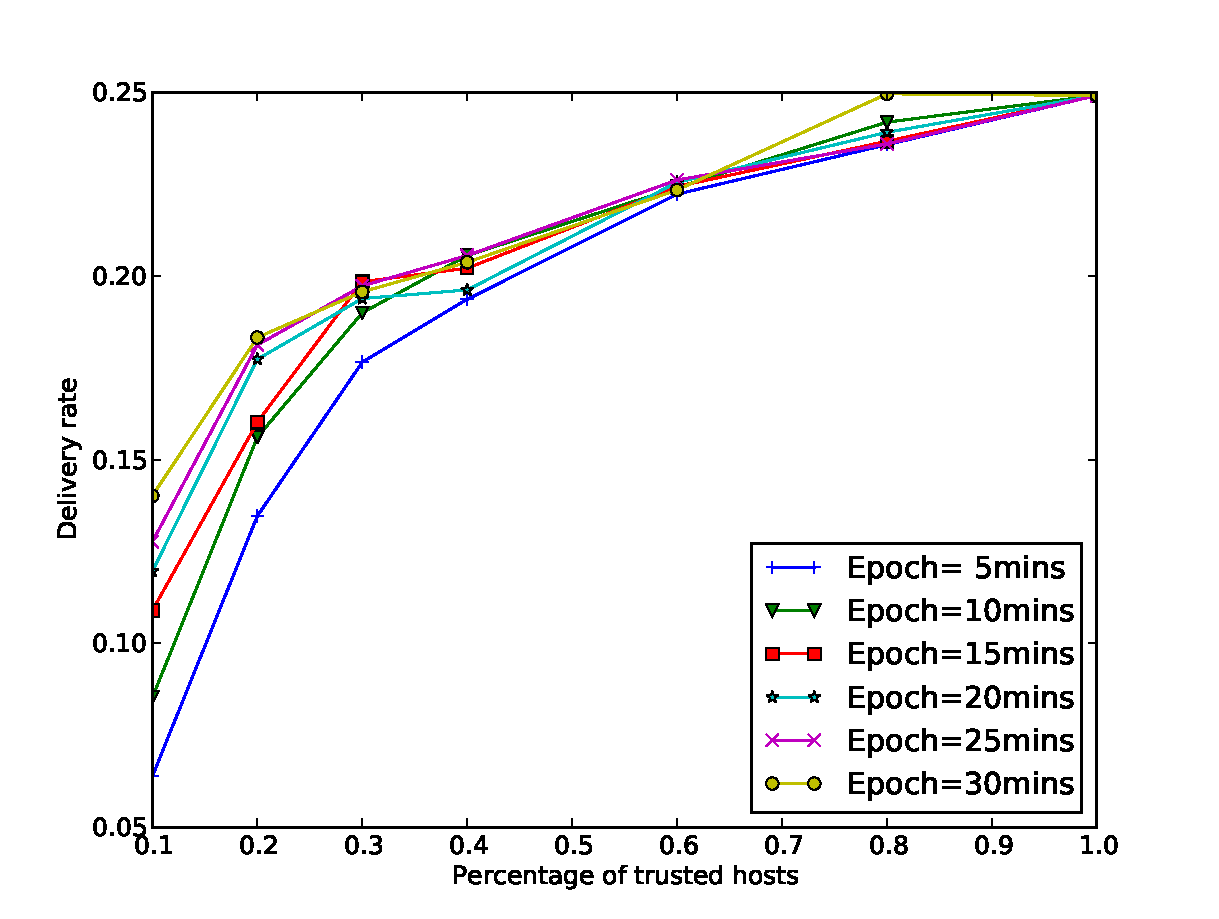
\includegraphics[width=0.6\columnwidth]{figures/delivery_rate.pdf}
\caption{{\bf Packet delivery rate (average of 3 trials).}
Percentage of trusted nodes affects packet delivery rate regardless of epoch. 
Epoch affects packet delivery rate only when the percentage of trusted nodes is less than $0.6$. 
In this simulation scenario, 10-min epoch seems to be reasonable, especially when percentage of trusted hosts $>= 0.3$.}
\label{fig:delivery_rate}
\end{figure}


\begin{figure}[h!]
\center
\subfloat[Packet delivery latency]{%
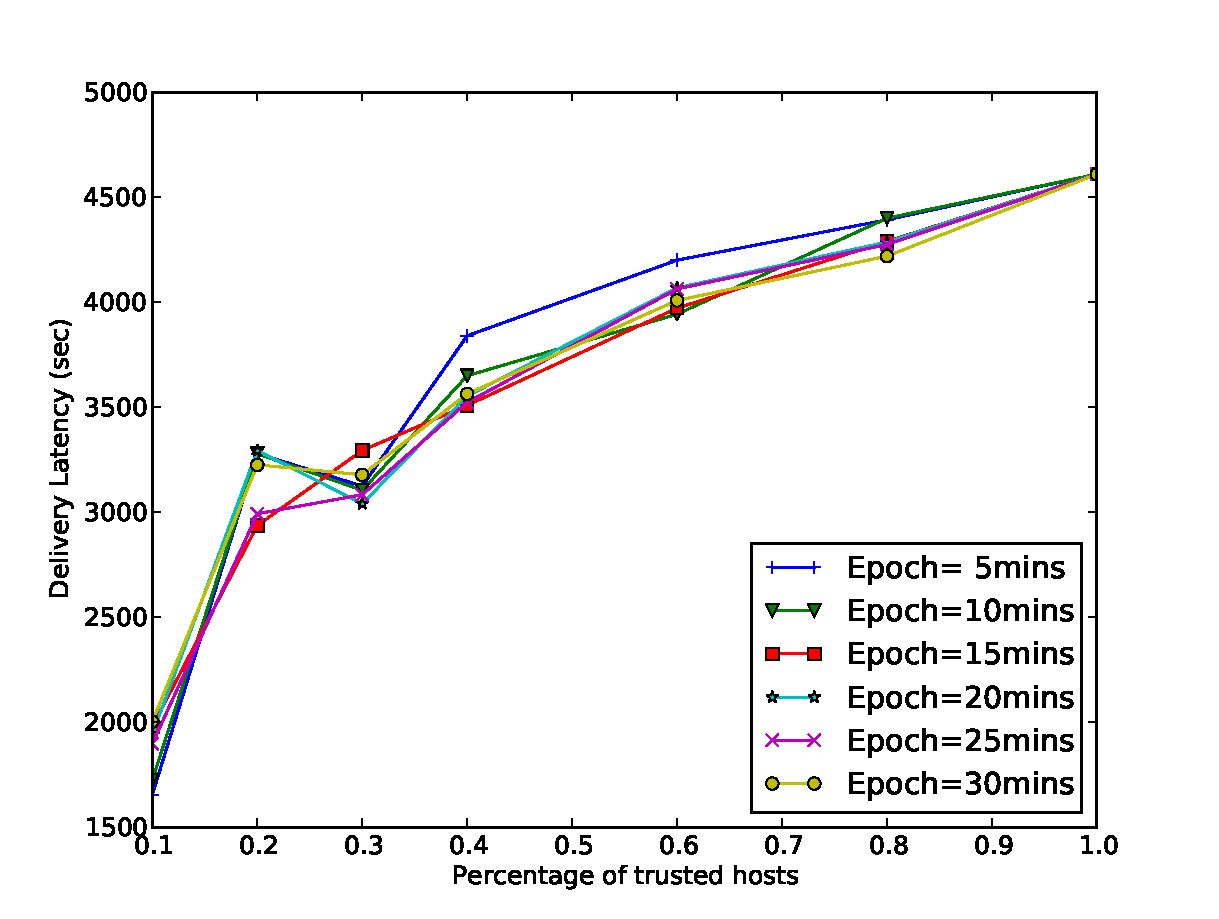
\includegraphics[width=0.49\columnwidth]{figures/latency.pdf}
\label{fig:latency}
}
\hfill
\subfloat[Packet delivery hop count]{%
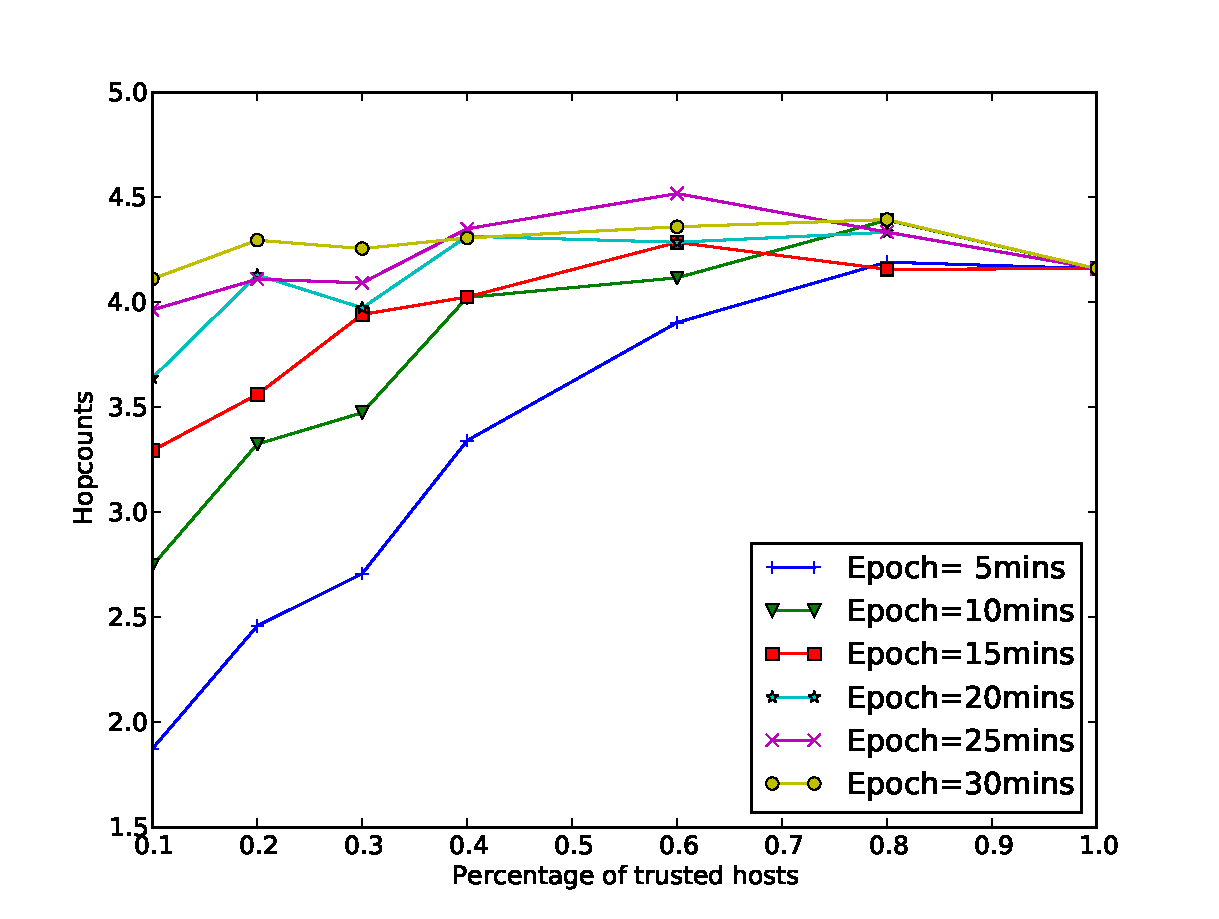
\includegraphics[width=0.49\columnwidth]{figures/hopcount.pdf}
\label{fig:hopcount}
}
\caption{{\bf Packet delivery latency \& hop count (average of 3 trials).}
Epoch does not affect packet delivery latency while it affects packet delivery hop count.  
It is interesting that larger hop count do not seem to increase delivery latency. 
}
\label{fig:delivery_latency_hopcount}
\end{figure}



\begin{figure}[h!]
\center
\subfloat[Relay classification over varied epoch. Percentage of trusted nodes = 0.3]{%
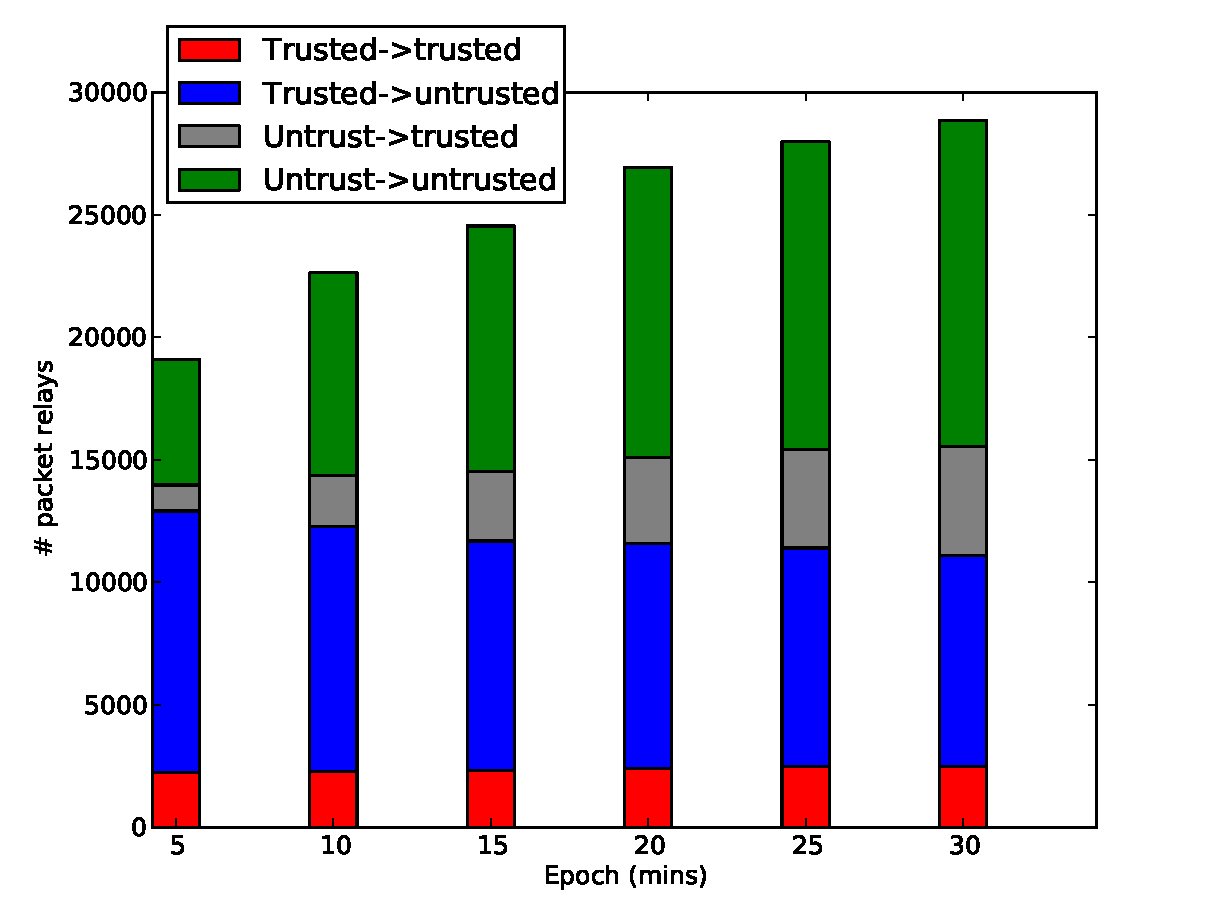
\includegraphics[width=0.49\columnwidth]{figures/relay_classification_over_epoch.pdf}
\label{fig:relay_classification_1}
}
\hfill
\subfloat[Relay classification over varied percentage of trusted nodes. Epoch = 10mins.]{%
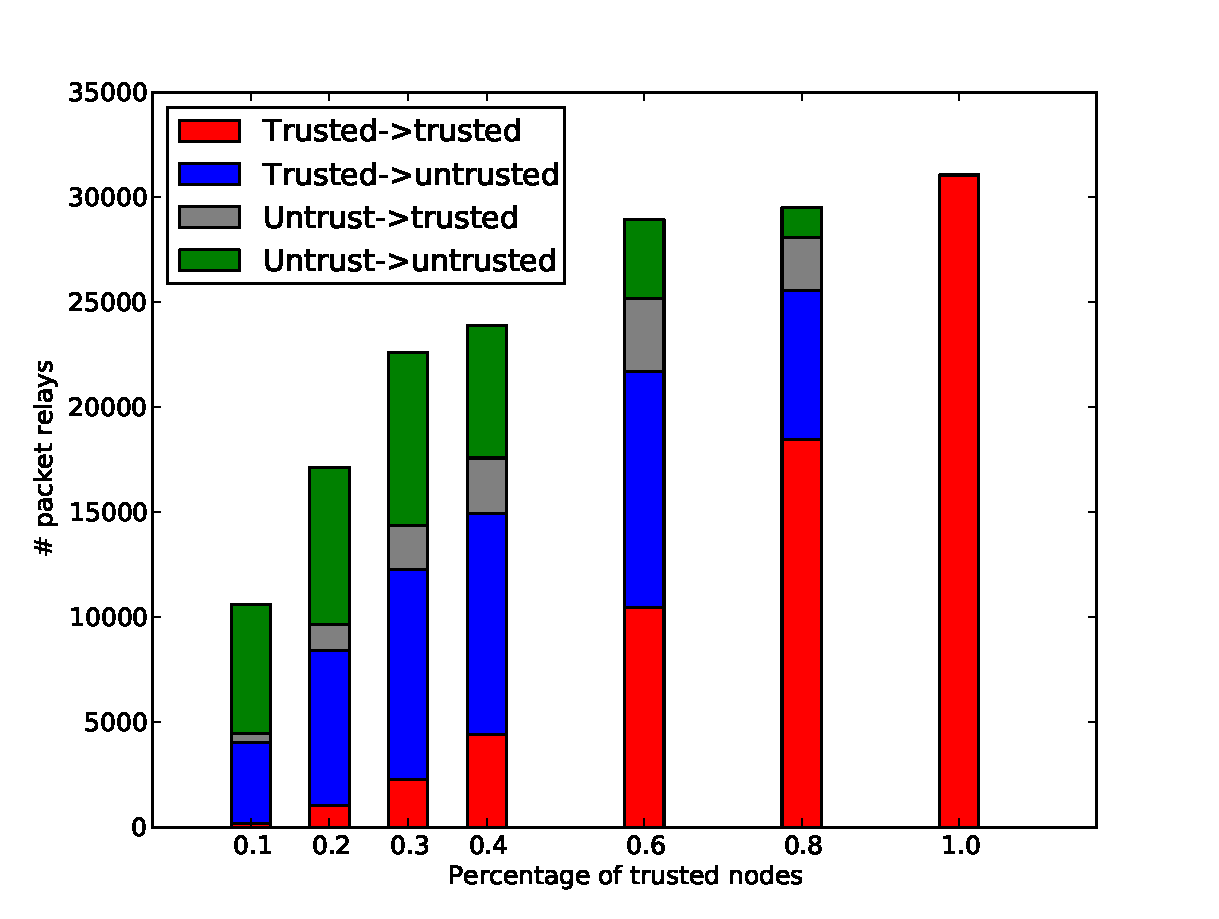
\includegraphics[width=0.49\columnwidth]{figures/relay_classification_over_percentage.pdf}
\label{fig:relay_classification_2}
}
\caption{{\bf Packet relay classification.}
Larger epoch increases relays from untrusted to trusted hosts and from untrusted to trusted host.  But it does not increase relays from trusted to trusted hosts.
Increasing percentage of trusted nodes generally increases relays from trusted to trusted nodes.
}
\label{fig:relay_classification}
\end{figure}






\begin{figure}[h!]
\center
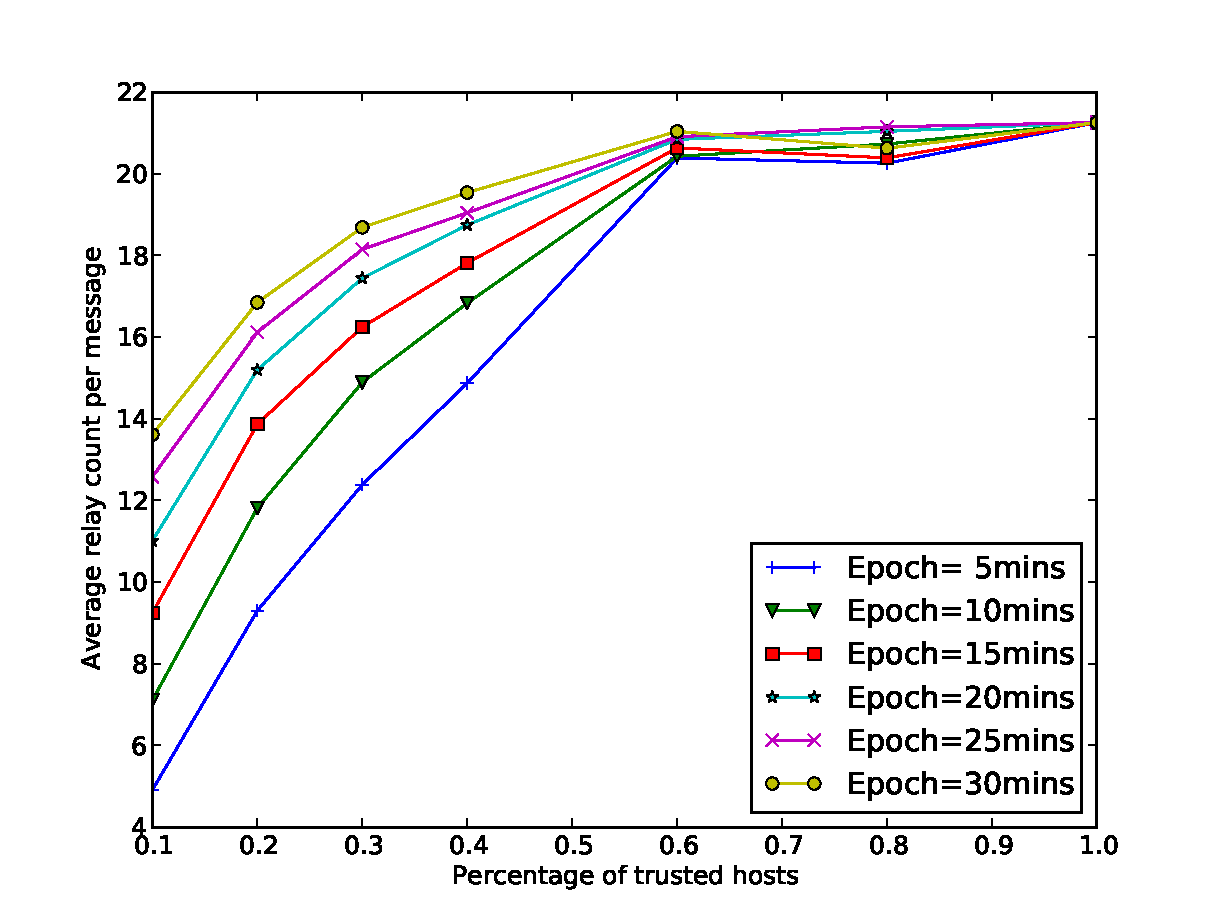
\includegraphics[width=0.6\columnwidth]{figures/average_relay_count.pdf}
\caption{{\bf Average relay counts per message (average of 3 trials).}
Packets are relayed similar times when percentage of trusted node $>= 0.6$, regardless of epoch.  
When percentage of trusted node $<0.6$, average relay count per message are directly effected by both epoch and percentage of trusted nodes. 
}
\label{fig:relay_count}
\end{figure}



\begin{figure}[h!]
\center
\subfloat[Packet drops over varied epoch. Percentage of trusted nodes = 0.3]{%
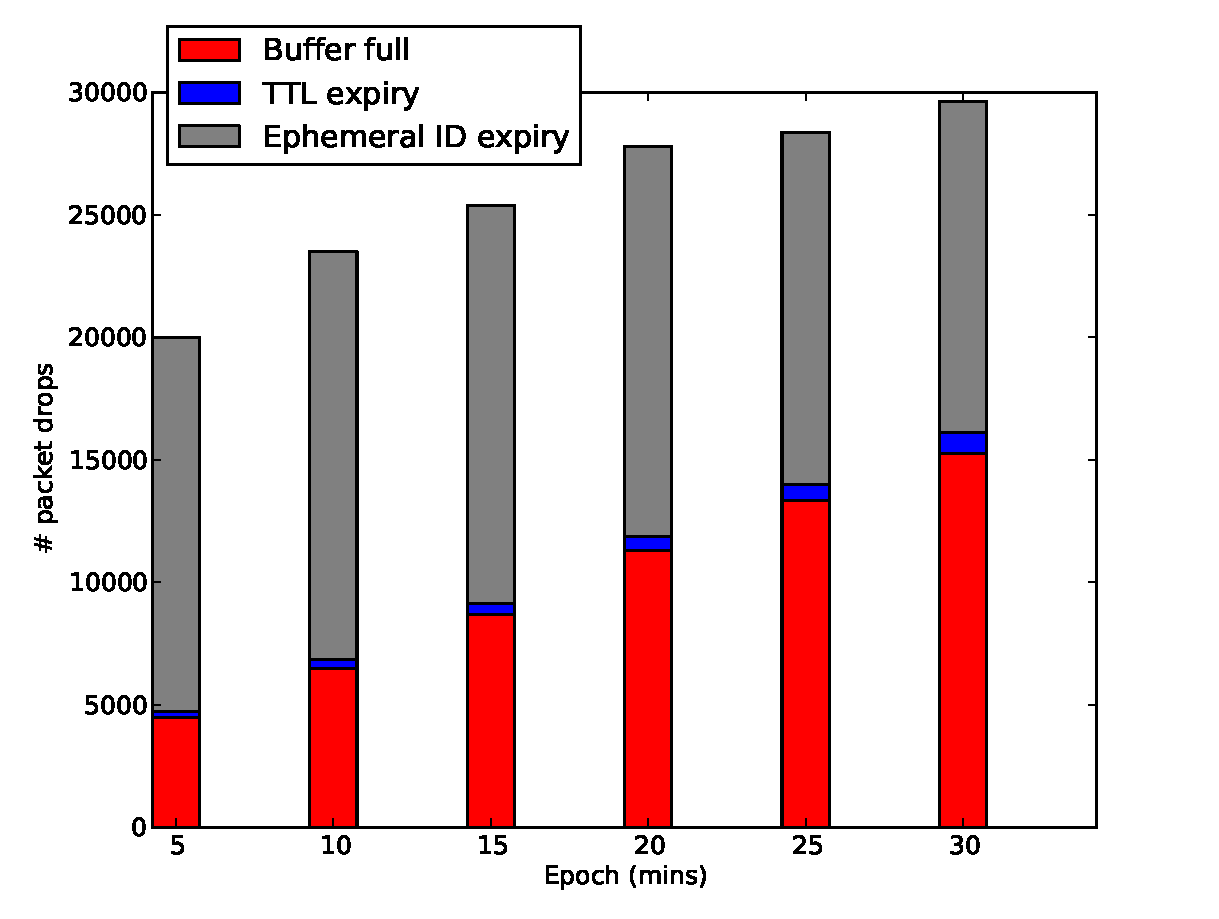
\includegraphics[width=0.49\columnwidth]{figures/drop_classification_over_epoch.pdf}
\label{fig:drop_classification_1}
}
\hfill
\subfloat[Packet drops over varied percentage of trusted nodes. Epoch = 10 mins.]{%
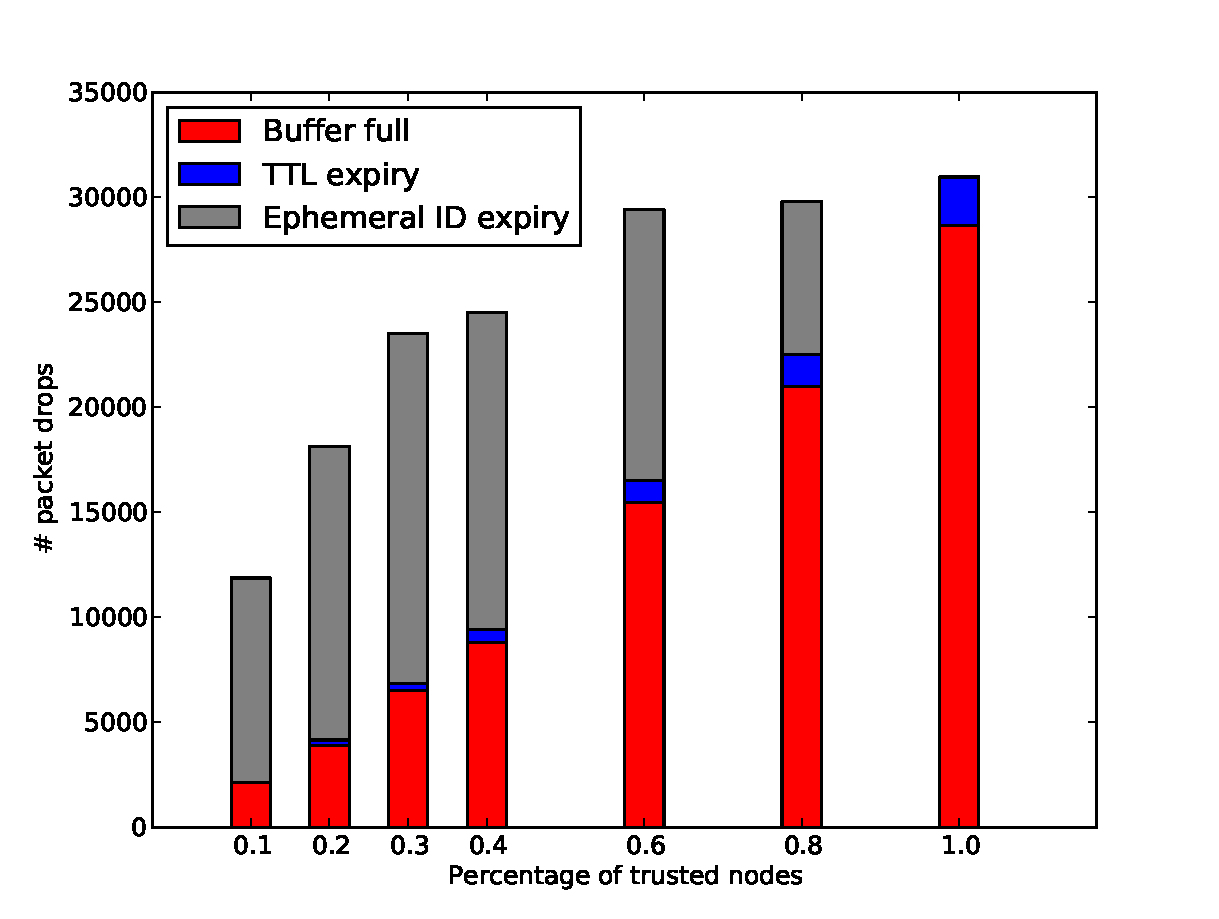
\includegraphics[width=0.49\columnwidth]{figures/drop_classification_over_percentage.pdf}
\label{fig:drop_classification_2}
}
\caption{{\bf Packet drop classification.}
With the fixed percentage of trusted nodes (0.3), larger epoch obviously increases packet drops due to buffer overflow, since it also means packets live in DTN for longer times.
With the fixed epoch (10 mins), larger percentage of trusted nodes increases packet drops due to buffer overflow and ephemeral ID expiry when percentage of trusted nodes $<=0.6$.
}
\label{fig:drop_classification}
\end{figure}







\begin{figure}[t!]
\center
\subfloat[Packet delivery count over varied epoch. Percentage of trusted nodes = 30]{%
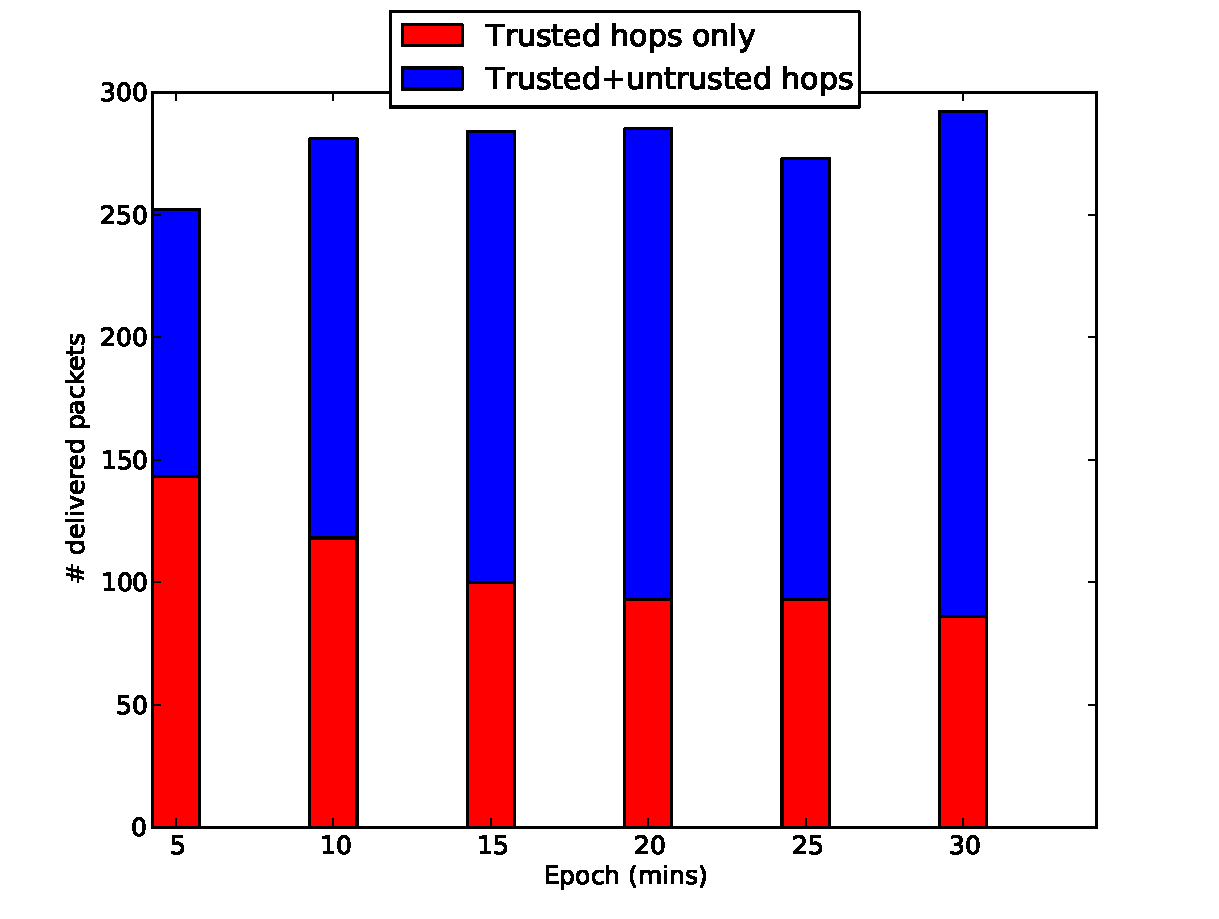
\includegraphics[width=0.49\columnwidth]{figures/delivery_count_over_epoch.pdf}
\label{fig:delivery_count_1}
}
\hfill
\subfloat[Packet delivery count over varied percentage of trusted nodes. Epoch = 10mins.]{%
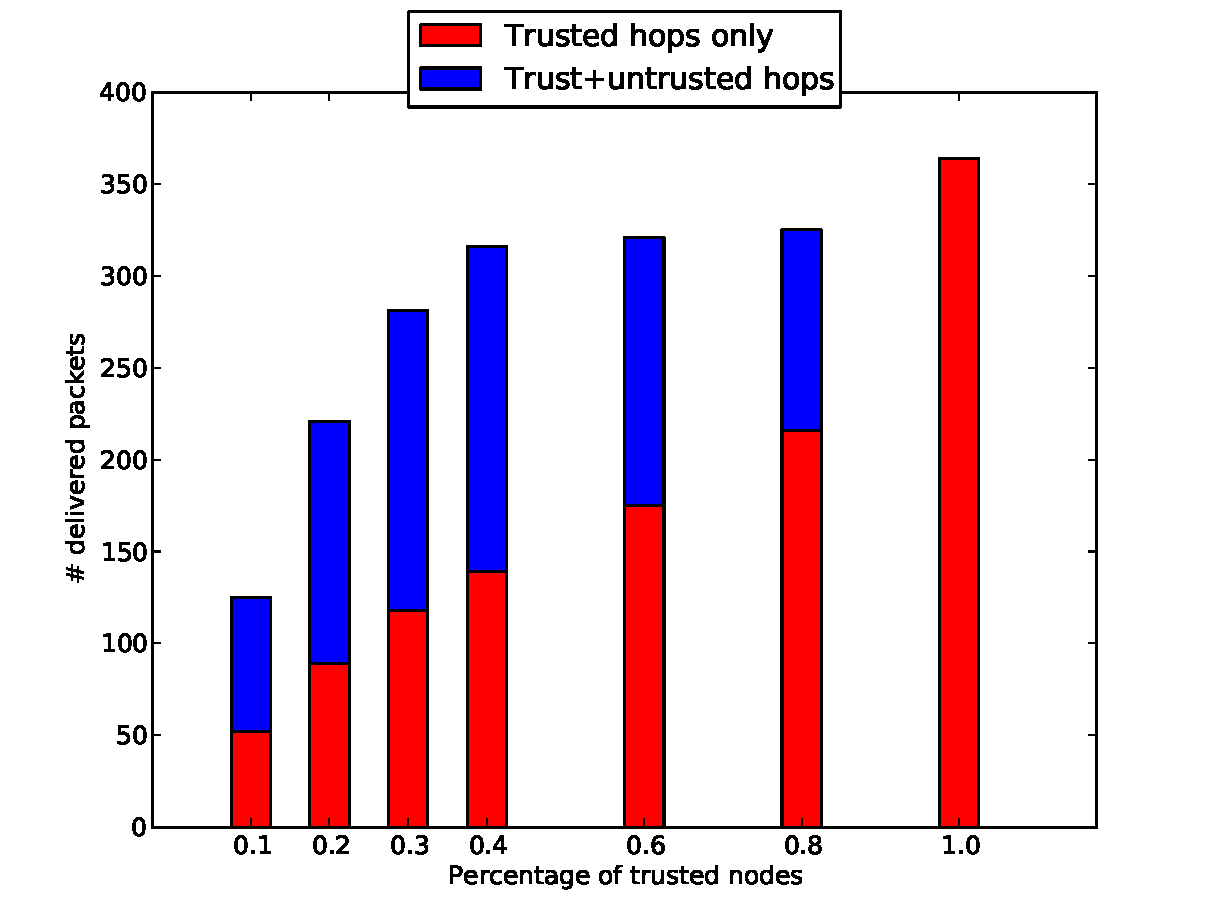
\includegraphics[width=0.49\columnwidth]{figures/delivery_count_over_percentage.pdf}
\label{fig:delivery_count_2}
}
\caption{{\bf Packet delivery count.}
Increasing epoch increases packet delivery count consists of trusted and untrusted hops.  Increasing percentage of trusted nodes increases packet delivery count with trusted hops only as well as that with trusted and untrusted hops while percentage of trusted nodes is less than $0.6$.
}
\label{fig:delivery_count}
\end{figure}





\end{document}







